
\chapter{Methods}

\label{Methods} 

This chapter describes in detail the methods for whatever activities were necessary for your project – e.g., data gathering, data analysis, requirements analysis, design, implementation, testing/evaluation, etc. Your choice of methods should be discussed and justified in view of the project objectives, and with reference to the pertinent literature. Report not only what methods you applied in generic terms, but what you actually did: sufficient information about dates and details for your reader to understand how you ran your project, rather than just how one could run any similar project.  

Report in this chapter what you did, not what you produced or found as a 
result (which goes under Results).  
  
Note: only use the word ‘methodology’ if you know what it means!  

%% On RELU not actually being differentiable:
%Some of the hidden units included in this list are not actually differentiable %at
%all input points. For example, the rectified linear function g (z) = max{0, z} is not
%differentiable at z = 0. This may seem like it invalidates g for use with a gradientbased
%learning algorithm. In practice, gradient descent still performs well enough
%for these models to be used for machine learning tasks. This is in part because
%neural network training algorithms do not usually arrive at a local minimum of
%the cost function, but instead merely reduce its value significantly,
%Because we do not
%expect training to actually reach a point where the gradient is 0 , it is %acceptable
%for the minima of the cost function to correspond to points with undefined gradient.
%Hidden units that are not differentiable are usually non-differentiable at only a
%small number of points.
% pg 207 Goodfellow
% This section from same book pg 475, maybe better in Context
%Another important push, still ongoing, has been towards end-to-end deep
%learning speech recognition systems that completely remove the HMM. The first
%major breakthrough in this direction came from Graves et al. (2013) who trained
%a deep LSTM RNN (see section 10.10), using MAP inference over the %frame-tophoneme
%alignment, as in LeCun et al. (1998b) and in the CTC framework (Graves
%et al., 2006; Graves, 2012).

% Batch normalization - in the context of preprocessing data for our trainng

\cite{ioffe2015batch, 7005077}
define Internal Covariate Shift as the change in the
distribution of network activations due to the change in
network parameters during training. To improve the training, we seek to reduce the internal covariate shift. By
fixing the distribution of the layer inputs x as the training
progresses, we expect to improve the training speed. I
"It has
been long known (LeCun et al., 1998b; Wiesler \& Ney,
2011) that the network training converges faster if its inputs are whitened – i.e., linearly transformed to have zero means and unit variances, and decorrelated. "
However, since x is affected by
W, b and the parameters of all the layers below, changes
to those parameters during training will likely move many
dimensions of x into the saturated regime of the nonlinearity and slow down the convergence. This effect is
amplified as the network depth increases.
 In practice,
the saturation problem and the resulting vanishing gradients are usually addressed by using Rectified Linear Units
(Nair \& Hinton, 2010) ReLU(x) = max(x, 0), careful
initialization (Bengio \& Glorot, 2010; Saxe et al., 2013),
and small learning rates. If, however, we could ensure
that the distribution of nonlinearity inputs remains more
stable as the network trains, then the optimizer would be
less likely to get stuck in the saturated regime, and the
training would accelerate.

\cite{lecun2012efficient}
Lecun points out:
Stochastic learning is usually much faster than batch learning, results in better solutions, particularly on large redundant datasets. The idea being since there is a lot of repetition (similar frames is dataset). SGD also works well because nonlinear networks usually have multiple local minima of different depths. The noise present in the updates can results jumping into the basin of another, possibly deeper, local minimum. Networks learn the fastest from the most unexpected sample, so examples should be chosen with the maximum information content by means of shuffling the training set, however care must be taken not to apply this technique with data that contains outliers

In the case of "In Bengio et al.’s paper [6], the analysis of the problem of gradient decays
is generalized to parameterized dynamical systems (hence including second
order and other recurrent architectures)" \cite{hochreiter2001gradient}
% LC - 14 pages

\section{Driving simulators}

Two driving simulators were trialed, an earlier version of Udacity (\cite{UdacityCarSim}) and SDSandbox (\cite{SDSandboxSim}). Both use the Unity game engine. The former had a large user base on account of the accompanying MOOC (Massive Online Open Course), which has since started using the Unreal (\cite{unrealengine}) based Carla (\cite{Dosovitskiy17}) sim. SDSandbox is actively developed for the \cite{DonkeyCar2020} and used by the do-it-yourself model-scale autonomous-vehicle community DIY Robocars (\cite{DIYRobocars2020}).
Both simulators are equivalent in the sense of acting as a data generator and also as a testing environment for self-driving CNNs. The difference being SDSandbox is able to generate data using, in addition to manual steering, a self-driving proportional–integral–derivative-like closed loop controller as implemented in PIDController.cs source code file. The feature makes generating training sets less laborious. The manual option being, a simulated car must be manually steered around the track a number of times to gather data. The process of gathering training data, manual or automated, creates a set of images and a set of corresponding steering angles, forming a labelled dataset.
The data is then moved from the output directory to a labelled directory of choice (details in appendix).



Both legacy Udacity and SDSandbox also run in autonomous driving modes (Fig. \ref{fig:UdacitySdSandboxAutonomous}).

\begin{figure}[h!]
\centering
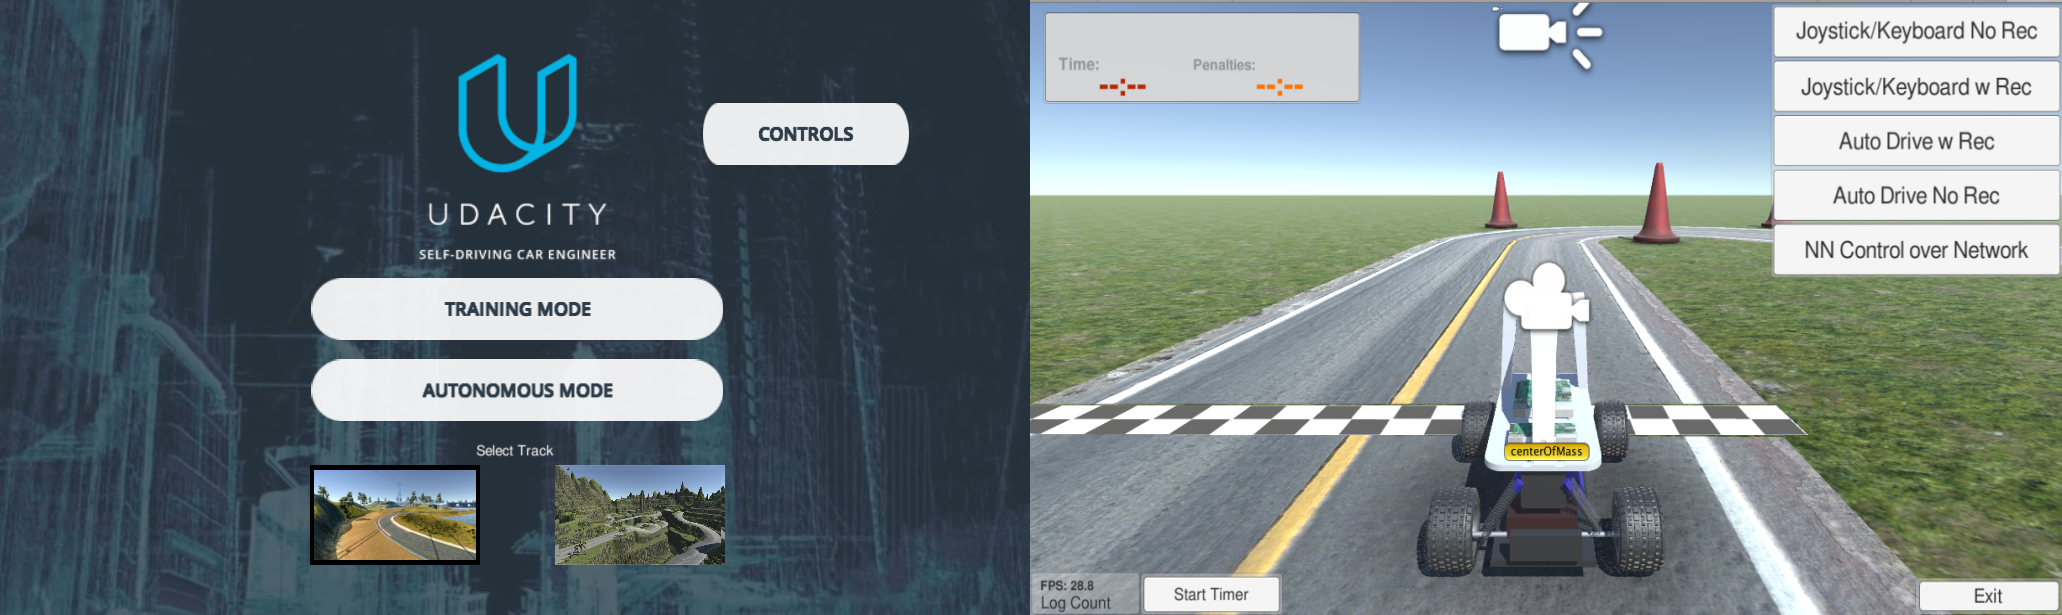
\includegraphics[scale=0.22]{UdacitySdSandboxSim.png}
\caption{Left to right: legacy Udacity and SDSandbox Autonomous Driving menus}
\label{fig:UdacitySdSandboxAutonomous}
\end{figure}

Setting up the simulator and prediction engine is further detailed in Appendix


\ref{RunningCarSimulatorForInference}.

\section{Data Augmentation}
To avoid overfitting, the data is augmented by: cropping the image to a height band that excluded horizon and car shadow, resized to required model input size, converted from RGB to YUV, 
% get images from http://localhost:8890/notebooks/augument.ipynb


\section{Development environments}

Models were created in different environments to accomodate the heavy workload. Intel DevCloud 

\subsection{Digital Images}
Digital images are stored as a square multidimensional matrix. A 100x100 colour images (with values from Red, Green and Blue) is represented as a matrix of dimensions $n x m x c$, where n is the width, m is the height and c is the depth (number of colour channels of the image. Black and white images have c = 1, where the pixel value is either on or off (TBC). Greyscale images also have one channel.

\subsection{Data Augmentation and Pre-Processing}

For the NVIDIA baseline model, assumed image capture size is 320wx160h pixels (to be confirmed), and the 200wx66h pixel image presented to network is a crop containing road and excluding horizon. The sequence shown in figure \ref{fig:augpreproc} presents image array sizes at every step, from top left to bottom right, the image is loaded, augmented with random horizontal flip (with corresponding steering negated), random shifts (with steering adjusted by adding or subtracting 0.002 degrees per shifted pixel, random addition of shadows and random modification of brightness. The image is then cropped to remove car and horizon, resized to the dimensions determined by network design (200x66 pixels for baseline network) and finally moved from RGB to YUV space.

\begin{figure}[ht]
 \centering 
 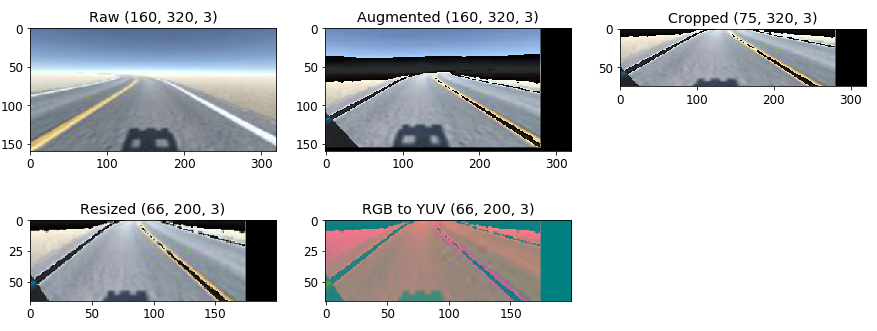
\includegraphics[width=\textwidth]{Figures/AugmentationPreProcessing.png}
 \caption{Stages of image augmentation and pre-processing with array dimensions on each step}
 \label{fig:augpreproc}
\end{figure}

Prior to presenting pixel colour channel values to the network, a number of pre-processing steps have become standard with neural network classifiers and regressors applied to computer vision.


Explain:  
\begin{itemize}
    \item Convolution
    \item pre-processing
    \item Kernel/filter size
    \item Stride
    \item padding
    \item activation function
    \item Loss function
    \item optimisers
    \item Back-propagation
    % on this topic, a lot to cite, from Paul Werbos' PhD thesis "Beyond Regression: New Tools for Prediction and Analysis in the Behavioural Sciences, through Rummelhart et al. and LeCunn et al.
\end{itemize}

Maybe cite goodfellow once and do a joblot on items.  

Our NVIDIA architecture is very similar to the one proposed by Bojarski et al. 2016. Our alternative AlexNet, GoogleLeNet, VGGNet and ResNet however have much fewer parameters. This is due to the "degradation" problem, where the number of parameters is too large for the dataset, and the network fails to converge.

\section{Datasets}
% What datasets we used and what data was gathered
3 datasets where used. Udacity self-driving real life data, Unity 3D game engine data, and the same datasets with added rain. Figure X shows details of the data.

The datasets are downloaded via script (\cite{Sikar2020}) and structured according to environment (local, Camber or DevCloud).

Two data augmentation libraries were used: \cite{Naoki2016} to add random shifts, flips, crop and change images to YUV format (as per \cite{bojarski2016end} data augmentation method used in the baseline architecture) and \cite{Saxena2017} to add rain and reflections to the testing datasets.

\section{Training and Testing}

The Keras (\cite{chollet2015keras}) deep learning API (Application Programming Interface) written in Python (\cite{van1995python}) and in this case acting as a wrapper around the machine learning library Tensorflow (\cite{abadi2016tensorflow})  was used to create, train and test models.

\subsection{Ford AV Dataset}
% Get details from https://avdata.ford.com/downloads/default.aspx
The Ford Autonomous Vehicle is a 
% angle from IMU
From % https://s23.q4cdn.com/258866874/files/doc_downloads/2020/03/2003.07969.pdf
 (\cite{Applanix}) is a professional-grade, compact,fully  integrated,  turnkey  position  and  orientation  system combining a differential GPS, an inertial measurement unit(IMU)  rated  with  1$^{\circ}$ of  drift  per  hour,  and  a  1024-count wheel encoder to measure the relative position, orientation,velocity,  angular  rate  and  acceleration  estimates  of  the vehicle. The Ford AV data set provides the 6-DOF pose (6DOF pose estimation of objects is the task of estimating the coordinates (X, Y,Z) and rotation angles (Yaw, Pitch and Roll) of an object with respect to a previously established reference coordinate system. (\cite{7005077} ) estimates obtained by integrating the (linear) acceleration and (angular) velocity.
% Note, Ford av authors discussion https://s23.q4cdn.com/258866874/files/doc_downloads/2020/03/2003.07969.pdf
% IEEE on 6DOF estimation from IMU discussion https://ieeexplore.ieee.org/document/7005077

% on converting GPS and IMU measurements to steering angles, see
% http://www.robesafe.uah.es/personal/roberto.arroyo/docs/Almazan13iv.pdf
% We might use a similar technique, time allowing

\subsection{Kitti}

The Kitti dataset TODO add provenance, add description
Data format, steering angle description obtained from oxts/dataformat.txt 
% cat 2011_09_26/2011_09_26_drive_0001_sync/oxts/dataformat.txt
\begin{verbatim}
yaw:   heading (rad),       0 = east,  positive = counter clockwise,\
    range: -pi   .. +pi
\end{verbatim}
Note, this may not be the steering angle - TBC. So additional work may be needed to obtain.
There are some pointers online, a simple approach seems to be:
% https://physics.stackexchange.com/questions/112301/calculating-the-rate-at-which-a-car-turns
This is also an interesting approach:
% http://docs.ros.org/en/kinetic/api/teb_local_planner_tutorials/html/cmd__vel__to__ackermann__drive_8py_source.html
With python code:
\begin{verbatim}
def convert_trans_rot_vel_to_steering_angle(v, omega, wheelbase):
  if omega == 0 or v == 0:
     return 0
  radius = v / omega
  return math.atan(wheelbase / radius)    
\end{verbatim}
Another possible method "Estimation of the Steering Angle Based on Extended Kalman-Filter"  
% http://gvpress.com/journals/IJMUE/vol11_no12/27.pdf
% equations 10 and 11

\subsection{Data balancing}

The data was found to be unbalanced, with most steering angles around the middle
\begin{figure}[ht]
 \centering 
 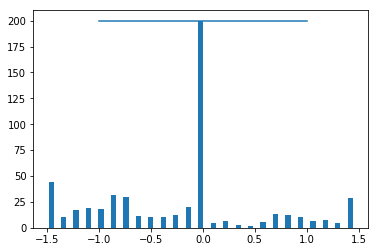
\includegraphics[scale=1]{Figures/bins.png}
 \caption{Diagram showing bins centered around zero degrees, meaning most of time car is driving straight. Binning diagrams for all datasets can be found in appendix B}
 \label{fig:bins-placeholder}
\end{figure}

\subsection{Data Augmentation}
The data was augmented with several methods

Describe was additional transformations was performed to enlarge dataset - maybe a discussion that more data is good? With references.


Found this article:
% https://lmb.informatik.uni-freiburg.de/Publications/2015/FDB15/image_orientation.pdf
Would some good suggestions:  
Augmentation. To prevent overfitting, we perform image augmentation, i.e., we
apply random transformations to input samples during network training on the
fly. We use translations (up to 5\% of the image width), brightness adjustment
% in the range [−0.2, 0.2], gamma adjustment with \\gamma \\memberof [−0.5, 0.1] and Gaussian
pixel noise with a standard deviation in the range [0, 0.02].
  
\section{Deep Convolutional Neural Network Models}

In this section all network architectures used are described.

\section{NVIDIA \textit{End to End Learning for Self-Driving Cars} Network Architecture}

The NVIDIA network (\ref{NVIDIA_baseline}) is the baseline sefl-driving architecture used in this study. This comprises three (RGB channel) x 66 (height) x 200 (width) size input layer corresponding to an image presented to network. The input layer is followed by: a normalization layer generating a 3 channel 66 x 200 layer, a 24 5x5 kernel convolutional layer generating 31x98 feature maps, a 36 5x5 kernel convolutional layer generating 14x47 feature maps, a 48 5x5 kernel convolutional layer generating 5x22 size feature maps, a 64 3x3 kernel convolutional layer generating 3x20 size feature maps, a 64 3x3 kernel generating 1x18 size feature maps, a 1164 neuron flattened layer fully connected to a 100 neuron layer, fully connected to a 50 neuron layer, fully connected to a 10 neuron layer, fully connected to a one neuron output layer.  
The first 3 convolutional layers have stride equal 2 and the last 2 convolutional layers have stride equal 1. Padding is equal to zero, resulting in smaller feature maps with every convolutional layer.
The size of feature maps generated by each convolutional layer is determined with equation \ref{eq:feature_map} as described in \cite{dumoulin2018guide}:
\begin{equation}
    \label{eq:feature_map}
    n_{out}= \Big\lfloor\frac{n_{in} + 2p -k}{s} \Big\rfloor +1
\end{equation}
where $n_{out}$ is output size of convolved feature map, $n_{in}$ is input size of image or feature map, $p$, $k$ and $s$ are padding, kernel and stride size respectively.  
 
For example, to determine size of feature maps in the first convolutional layer $n_{out}=\lfloor(66+(2\times0)-5)/2\rfloor)+1=31$, $n_{out}=\lfloor(200+(2\times0)-5)/2\rfloor+1=98$. The Keras (\cite{chollet2015keras}) machine learning framework is used to build the model. The calculation for number of trainable parameters (weights) in a convolutional layer is assumed to be:
\begin{equation}
    \label{eq:feature_map}
    n_p= m \times n \times  d \times k + d
\end{equation}
where $m$ and $n$ are the convolutional kernel dimensions, $d$ is the number of feature maps in the current layer and $k$ is the number of feature maps in the previous layer. Note $d$ is added to acccount for \textit{bias} term. For example, the number of trainable parameters for the first convolutional layer in \ref{NVIDIA_baseline} is given by $n_p = 5 \times 5 \times 24 \times 3 + 24 = 1,824$. The number of trainable parameters in a fully connected layer is given by:
\begin{equation}
    \label{eq:feature_map}
    n_p= m \times n + n
\end{equation}
where $m$ is the number of inputs in previous layer and $n$ is number of neurons in current layer. Note second term $n$ is added to account for \textit{bias} term. For example, for the first fully connected layer in \ref{NVIDIA_baseline} the number of parameters is given by $n_p = 1164 \times 100 = 1,342,092$, where the inputs are values from previous flattened layer, that is, a vectorized representation of the last convolutional layer feature maps.  
The total number of trainable parameters generated by Keras is 1,595,511. This does not agree with the total given by \cite{bojarski2016end}, who state their "network  has  about (...) 250 thousand parameters". Total memory required to store parameters assuming 32-bit float data type, is 6MB given by $1,595,511 \times 4 \div 1,024 \div 1,024$.

Since the NVIDIA model is based on work by \cite{krizhevsky2012imagenet}, "dropout" (\cite{hinton2012improving}) is assumed to have been used, with 50\% dropout probability on every layer.  
Dropout removes neurons randomly and helps prevent overfitting, where a model performs well on training data and poorly on testing data, by preventing co-adaptation, resulting in neurons that can detect useful features in the multitude of contexts it must operate, and help the network produce the correct answer.
As per correspondence with co-author(\ref{corr_with_authors} additional training hyperparameters are MSE (loss function) 
adadelta (optimizer), "learning rate: 1e-4 (but not really used in adadelta)" and 0.25 dropout.
Additional assumptions on training include: 128 example batch size, weights initialized from a zero-mean normal distribution with standard deviation 0.01 and biases mostly initialized to 1 as per \cite{krizhevsky2012imagenet}, which applied to this baseline architecture initializes all biases to 1, except in convolutional layers 1 and 5, where biases are initialized to 0. Details in source code src/models.py, nivia\_baseline function.  


% TODO need to incorporate section 5    Details of learning of Krizhesvky et al i.e.
%We trained our models using stochastic gradient descent with a batch size of 128 examples, momentum of 0.9, andw eight decay of 0.0005. ETC

% Since the weights are not initialized properly and groups of neurons end up in the same local minima, according to their (similar) initialization.
% To overcome this, you could use dropout / drop connect to break symmetry.
% https://stats.stackexchange.com/questions/181264/how-does-co-adaptation-occur-in-deep-neural-nets

% NB no reference to "Alexnet" in original or NVIDIA articles - clean up required.
%For example, in the classic Alexnet (\cite{krizhevsky2012imagenet}) architecture, with input %image size 224x224, kernel size 11, padding equal zero and stride = 4, the resulting feature %map size in the first convolutional layer is 55x55. 
%Alexnet has an input layer with dimensions 224x224x3, where 3 is the number of channels (RGB %image), the second layer has dimensions 55x55x48, the third convolutional layer has %dimensions 27x27x128 and so on. This is typical of deep network architectures, decreasing %feature map sizes with increasing number of channels as network depth increases.
`  

\textbf{Discussion on the number of parameters required given size of dataset.}  
We also need a discussion on deep regression models as suggested by \cite{lathuilire2018comprehensive}. This is the main difference between the NVIDIA and additional models, the NVIDIA model is a regression model while the models we compare and contrast with NVIDIA are classification models built specifically for the ILSVC  competitiion.

\subsection{ResNet}

Discuss the concept of "residuals". ResNet makes use of skip-connections (spelling), these "network architecture
designs (e.g., skip connections) produce loss functions that train easier", producing smoother loss surfaces (\cite{li2017visualizing})  
The "Degradation problem itself stems from the fact that it is easier to learn 0 than to learn 1"   https://www.youtube.com/watch?v=jio04YvgraU
"if an identity mapping were optimal, it would be easier to push the residual to zero than to fit an identity mapping by a stack of nonlinear layers" \cite{he2015deep}.  
Explain what variation A, B or C we will be using (zero padding, weights * x, etc.  
"Essemble" of ResNets was used.  
18 layers seems to be a threshold, beyond that, training becomes difficult. Skip connections make deeper networks, i.e. networks with more layers, easier to train compared to networks without skip connections.  
Another wording, deeper neural networks (i.e. layer count equal or greater than 20) become increasingly difficult to train, generating poorer accuracy than deep networks with less than 20 layers. This is known as "degradation problem" (citation needed). Skip connections make deeper architectures easier to train, by smoothing the loss function.

\subsection{GoogleLeNet}

This network (\cite{szegedy2014going}) was the winning entry in the ILSVCC 2014 Classification Challenge. It uses the LeNet-5 (\cite{Lecun98gradient-basedlearning}) model as a starting point, following the now traditional design of ConvNets with the addition of \textit{Inception} modules as introduced by \cite{lin2013network} in the \textit{Network in Network} model.

\begin{figure}[ht]
 \centering 
 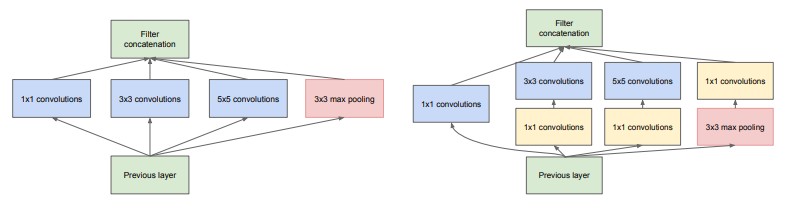
\includegraphics[width=\columnwidth]{Figures/InceptionModules.png}
 \caption{Inception naive (left) and dimension reduction model (right)}
 \label{fig:inception_modules}
\end{figure}

The designers of the GoogleLeNet architecture state that power and memory use is important to consider and aim to keep a computation budget of 1.5 billion multiply adds at inference time such that the resulting model could be used in practice at a reasonable cost.

The architecture contains 22 layers where all

\subsection{Deep Regression Models}
Explain the process of transforming these models (except NVIDIA) into regression models, maybe cite \cite{lathuilire2018comprehensive} or papers cited therein.

Paper is referred to by this discussion: 
% https://stats.stackexchange.com/questions/335836/cnn-architectures-for-regression
A somewhat more succinct definition of the procedure:  
% https://stats.stackexchange.com/questions/456126/could-resnet-curve-be-used-for-a-regression-problem-e-g-housing-price-predicti
Just to make it clear, a regression problem is one whose target is continuous and not discrete. In this sense you can make any Neural Network that is primarily used for classification a regressor, with minimal changes. Namely it needs to end with 1 neuron, no activation function and a proper loss function (e.g. mean squared error). For example, object detection is in its core a regression problem because you are trying to predict coordinates. Any ResNet could be used for these problems

\subsection{Binning/Quantization}
Describe this approach, if we get that far, to use an alternative to regression models, whereby we may bin the outputs. This could potentially simplify the model. Also, depending on track, we could have narrower bins around zero degrees, i.e. finer control and wider bins away from zero degrees, i.e. coarser control. Or vice-versa - experimentation required.

\subsection{Training}

We might want to add that training was done on AWS GPUs following   
https://aws.amazon.com/blogs/machine-learning/train-deep-learning-models-on-gpus-using-amazon-ec2-spot-instances/  


\section{Evalutation}
This section discussed the evaluation benchmarks, here we discuss the evaluation environment (Unity 3D game engine) and how it was used to both generate data and evaluate the models.

%% Udacity
%% see https://arxiv.org/pdf/1912.05440.pdf
%% for discussion on using rmse as error metric


